\begin{Example}
We are particularly interested in the case $\mathcal{V} = \Oq\text{-}{\rm comod}^{\rm fin}$, for which the relations the Reshetikhin--Turaev functor imposes (between framed tangles) are precisely the Kauffman-bracket relations.
\end{Example}

\begin{Remark}\label{rmkUnorTanOq}
In any skein category, the identity coupon ${\rm Id}_{X^*}\colon X^* \to X^*$ with entry a downward oriented $X$-coloured ribbon and output an upward oriented $X^*$-coloured ribbon depicted below gives an identification $(X,-) \simeq (X^*,+)$.
$$
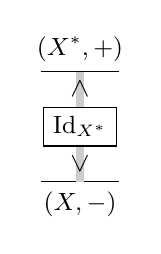
\begin{tikzpicture}[yscale = 0.7, baseline = 0pt]
\draw (0,0) -- (1,0) node[midway,below]{\small $(X,-)$};
\draw (0,2) -- (1,2) node[midway,above]{\small $(X^*,+)$};
\node[draw, rectangle] (I) at (0.5,1) {\small ${\rm Id}_{X^*}$};
\draw[gray!40, line width = 3pt] (0.5,0) -- (I) node[midway, sloped, black]{$<$} -- (0.5,2) node[midway, sloped, black]{$>$};
\end{tikzpicture}
$$
In the case $\mathcal{V} = \Oq\text{-}{\rm comod}^{\rm fin}$ and $X = V$ is the standard corepresentation, the object~$V^*$ is already isomorphic to $V$ in $\mathcal{V}$ by $\varphi$ from Definition~\ref{defOqcomods}. Thus one gets an identification $(V,+) \simeq (V,-)$ and sliding the coupon coloured by it along a strand changes the orientation of the strand. Consequently, one can switch signs of points and orientations of strands.
\end{Remark}

 In the following, we stop mentioning them and talk about unoriented framed tangles. The Reshetikin--Turaev functor is still well-defined on unoriented framed tangles, see \cite[Theorem~4.2]{Tingley}. An unoriented tangle gives a ribbon graph by choosing an arbitrary orientation, colouring every strand by $V$ and replacing $V^*$'s imposed on the boundary points by $V$'s using $\varphi$ or $\varphi^{-1}$. Concretely, for the unoriented cap $\cap$ for example, one can orient it either left or right, so one has to check that $\mathop{\rm RT}(\lcap) \circ (\varphi \otimes {\rm Id}_V) = \mathop{\rm RT}(\rcap) \circ ({\rm Id}_V \otimes \varphi)$. Note that this would not hold with the usual coribbon element in $\Oq$.

{\sloppy\begin{Theorem}[{\cite[Theorem~12.3.10]{CP}} or {\cite[Theorem~3.3.4]{Carter}} for endomorphisms in $\mathbb{R}^2$]\label{thmSkAsTangles}
Let~$n.V$ and~$m.V$ be two objects of ${\rm Sk}_\mathcal{V}(\Sigma)$ given respectively by $n$ and $m$ points coloured by $V$. Then any morphism in $\Hom_{{\rm Sk}_\mathcal{V}(\Sigma)}(n.V,m.V)$ can be represented by a linear combination of unoriented framed tangles $($without coupons$)$. Moreover, two linear combinations of unoriented framed tangles represent the same morphism in $\Hom_{{\rm Sk}_\mathcal{V}(\Sigma)}(n.V,m.V)$ if and only if one can get from one to the other by a~sequence of isotopies and Kauffman-bracket relations.
\end{Theorem}}

\begin{Corollary}
The algebra $\Hom_{{\rm Sk}_\mathcal{V}(\mathbb{R}^2)}(n.V,n.V)$ is isomorphic to the Temperley--Lieb algebra~${\rm TL}_n$, defined in {\rm \cite[Section~XII.3]{Turaev}}. The full subcategory of ${\rm Sk}_\mathcal{V}\big(\mathbb{R}^2\big)$ of objects of the form~$[n]$ with every point coloured by $V$ is equivalent to the category ${\rm TL}$, defined in {\rm\cite[Section~XII.2]{Turaev}}. In the following, we will call this full subcategory ${\rm TL}$.
\end{Corollary}

The category ${\rm TL}$ is a ribbon full subcategory of $\mathcal{V}$, and the above theorem proves that for any surface $\Sigma$ the category ${\rm Sk}_{{\rm TL}}(\Sigma)$ is a full subcategory of ${\rm Sk}_\mathcal{V}(\Sigma)$.

\subsection{Stated skein algebras}\label{SectStatedSkein} Stated skein algebras generalise skein algebras for tangles on a marked surface with boundary, see \cite{BonahonWong,TTQLe,Muller}. These tangles can be cut and stated skein algebras satisfy nice excision properties. We will recall here the approach of \cite{Cos}. Stated skein algebras can be defined over integral rings of coefficients, but we will work over a field $k$ being either $\mathbb{Q}\big(q^{\frac{1}{2}}\big)$ or $\mathbb{C}$ with $q^{\frac{1}{2}} \in \mathbb{C}^\times$ generic, as our proofs only hold in this context.

\begin{Definition}
Let $\mathfrak{S}$ be an oriented surface. The skein algebra $\mathring{\mathscr{S}}(\mathfrak{S})$ is the $k$-vector space generated by isotopy classes of unoriented framed links in $\mathfrak{S}\times (0,1)$ modulo the skein relations:
\[ \Kauftresse \ = q \Kaufvert\ +q^{-1} \Kaufhoriz \qquad \text{and} \qquad \Kaufcirc \ = \big({-}q^2-q^{-2}\big) \Kaufvide \]
in a little embedded cube $\phi\colon \mathbb{D}^3 \hookrightarrow \mathfrak{S}\times (0,1)$.

It is an algebra with product given by vertical superposition $\mathfrak{S}\times (0,1) \sqcup \mathfrak{S}\times (0,1) \overset{\left(\frac{1}{2},1\right)\sqcup\left(0,\frac{1}{2}\right)}\longrightarrow \mathfrak{S} \times (0,1)$ and unit the empty link.
\end{Definition}

Note that by Theorem~\ref{thmSkAsTangles}, one has an algebra isomorphism
\[
\mathring{\mathscr{S}}(\mathfrak{S}) \simeq \End_{{\rm Sk}_{\Oqcomfin}(\Sigma)}(\varnothing).
\]

\begin{Definition}
A marked surface is a compact oriented surface with boundary $\overline{\mathfrak{S}}$ with a finite set $P\subseteq \partial\overline{\mathfrak{S}}$ of boundary points, called marked points. We write $\mathfrak{S} = \overline{\mathfrak{S}} \smallsetminus P$ and call this the marked surface. We write $\partial_P\overline{\mathfrak{S}}$ the boundary components of $\overline{\mathfrak{S}}$ that contain a point of $P$ and $\partial \mathfrak{S} := \partial_P\overline{\mathfrak{S}} \smallsetminus P$. Namely we only consider boundary components of $\mathfrak{S}$ that contain a marked point, which we remove in $\mathfrak{S}$, so all components of $\partial \mathfrak{S}$ are intervals. The circular boundary components are discarded and give punctures in $\mathfrak{S}$. The boundary structure of stated skein algebras will depend on a way to cut out a bigon out of a~boundary edge, and that of internal skein algebras on a way to insert one from a~boundary edge. To avoid choices, we suppose that marked surfaces come equipped with a thickening of their boundary edges inside the surface.

A stated tangle $\alpha$ on $\mathfrak{S}$ is an unoriented, framed, compact, properly embedded 1-submanifold of $\mathfrak{S} \times (0,1)$ whose boundary $\partial \alpha \subseteq \partial\mathfrak{S} \times (0,1)$ has positively vertical framing and comes equipped with a~state ${\rm st}\colon \partial \alpha \to \{+,-\}$. We call height the $(0,1)$-coordinate of a point, and require that all boundary points of $\alpha$ lying over a same component of $\partial\mathfrak{S}$ have distinct heights. An isotopy of stated tangles is an isotopy with values in stated tangles, in particular preserving the height order over a same boundary component. A stated tangle in $\mathfrak{S} \times (0,1)$ can always be represented as a diagram with blackboard framing in $\mathfrak{S}$, with its under/over crossing information, such that the height order of boundary points corresponds to a given orientation on the boundary edges, see \cite[Section~3.5]{BonahonWong}.
\end{Definition}

\begin{Definition}[{\cite[Section~2.5]{Cos}}]
The stated skein algebra $\mathscr{S}(\mathfrak{S})$ of a marked surface $\mathfrak{S}$ is the $k$-vector space generated by isotopy classes of stated tangles on $\mathfrak{S}$ modulo usual skein relations:
\[
\Kauftresse \ = q \Kaufvert\ + q^{-1} \Kaufhoriz\,, \qquad
\Kaufcirc \ = \big({-}q^2-q^{-2}\big)\, \Kaufvide\
\]
and the boundary skein relations:
\[
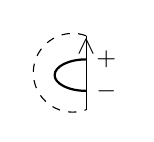
\begin{tikzpicture}[scale = 0.5, baseline = -3pt]
\draw[dashed] (70:1) arc(70:290:1);
\draw (-70:1) -- (70:1) node[pos = 0.85,sloped]{\small $>$};
\draw[thick] (70:1)++ (0,-0.6) node[right]{\small $+$} arc(90:270:0.8 and 0.4) node[right]{\small $-$};
\end{tikzpicture}
= q^{-\frac{1}{2}} \begin{tikzpicture}[scale = 0.5, baseline = -3pt]
\draw[dashed] (70:1) arc(70:290:1);
\draw (-70:1) -- (70:1) node[pos = 0.85,sloped]{\small $>$};
\end{tikzpicture}\!, \qquad
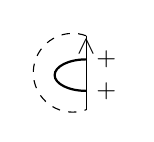
\begin{tikzpicture}[scale = 0.5, baseline = -3pt]
\draw[dashed] (70:1) arc(70:290:1);
\draw (-70:1) -- (70:1) node[pos = 0.85,sloped]{\small $>$};
\draw[thick] (70:1)++ (0,-0.6) node[right]{\small $+$} arc(90:270:0.8 and 0.4) node[right]{\small $+$};
\end{tikzpicture} = 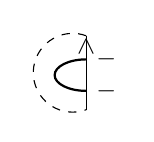
\begin{tikzpicture}[scale = 0.5, baseline = -3pt]
\draw[dashed] (70:1) arc(70:290:1);
\draw (-70:1) -- (70:1) node[pos = 0.85,sloped]{\small $>$};
\draw[thick] (70:1)++ (0,-0.6) node[right]{\small $-$} arc(90:270:0.8 and 0.4) node[right]{\small $-$};
\end{tikzpicture} = 0,
\qquad
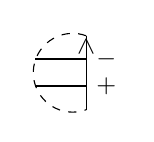
\begin{tikzpicture}[scale = 0.5, baseline = -3pt]
\draw[dashed] (70:1) arc(70:290:1);
\draw (-70:1) -- (70:1) node[pos = 0.85,sloped]{\small $>$};
\draw[thick] (70:1)++ (0,-0.6) node[right]{\small $-$} -- ++(-1.3,0);
\draw[thick] (-70:1)++ (0,0.6) node[right]{\small $+$} -- ++(-1.3,0);
\end{tikzpicture}
=q^2 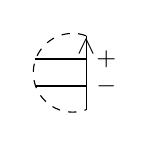
\begin{tikzpicture}[scale = 0.5, baseline = -3pt]
\draw[dashed] (70:1) arc(70:290:1);
\draw (-70:1) -- (70:1) node[pos = 0.85,sloped]{\small $>$};
\draw[thick] (70:1)++ (0,-0.6) node[right]{\small $+$} -- ++(-1.3,0);
\draw[thick] (-70:1)++ (0,0.6) node[right]{\small $-$} -- ++(-1.3,0);
\end{tikzpicture}
+q^{-\frac{1}{2}} 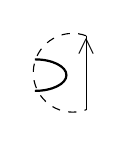
\begin{tikzpicture}[scale = 0.5, baseline = -3pt]
\draw[dashed] (70:1) arc(70:290:1);
\draw (-70:1) -- (70:1) node[pos = 0.85,sloped]{\small $>$};
\draw[thick] (70:1)++ (-1.3,-0.6) arc(90:-90:0.8 and 0.4);
\end{tikzpicture}\!,
\]
where the arrows on the boundary edges represent the relative height order of the two points.
It is an algebra with product given by vertical superposition and unit the empty link.

We denote by $C^\mu_\nu$ the coefficient such that
\[
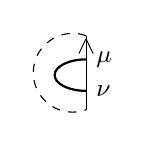
\begin{tikzpicture}[scale = 0.5, baseline = -3pt]
\draw[dashed] (70:1) arc(70:290:1);
\draw (-70:1) -- (70:1) node[pos = 0.85,sloped]{\small $>$};
\draw[thick] (70:1)++ (0,-0.6) node[right]{\small $\mu$} arc(90:270:0.8 and 0.4) node[right]{\small $\nu$};
\end{tikzpicture} = C^\mu_\nu \begin{tikzpicture}[scale = 0.5, baseline = -3pt]
\draw[dashed] (70:1) arc(70:290:1);
\draw (-70:1) -- (70:1) node[pos = 0.85,sloped]{\small $>$};
\end{tikzpicture},
\]
namely $C_+^+ = C_-^- = 0$, $C^+_-=q^{-\frac{1}{2}}$ and one can compute $C^-_+ = -q^{-\frac{5}{2}}$, see \cite[Lemma~2.3(13)]{Cos}. We~also write $C(\nu) := C_\nu^{-\nu}$.
\end{Definition}

\begin{Proposition}[{\cite[Lemmas 2.3 and 2.4]{TTQLe}}] \label{propLeftStSkRel}
These relations express equivalently with the boundary at the left, namely:
\[
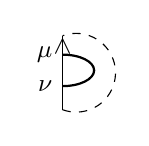
\begin{tikzpicture}[scale = 0.5, baseline = -3pt, rotate = 180]
\draw[dashed] (70:1) arc(70:290:1);
\draw (-70:1) -- (70:1) node[pos = 0.15,sloped]{\small $>$};
\draw[thick] (70:1)++ (0,-0.6) node[left]{\small $\nu$} arc(90:270:0.8 and 0.4) node[left]{\small $\mu$};
\end{tikzpicture} = {}^{\mu}_{\nu}\reflectbox{$C$} \begin{tikzpicture}[scale = 0.5, baseline = -3pt, rotate = 180]
\draw[dashed] (70:1) arc(70:290:1);
\draw (-70:1) -- (70:1) node[pos = 0.15,sloped]{\small $>$};
\end{tikzpicture},
\]
where ${}^+_+ \reflectbox{$C$} = {}^-_-\reflectbox{$C$}=0$, ${}^+_-\reflectbox{$C$}= -q^{\frac{5}{2}}$ and ${}^-_+\reflectbox{$C$}= q^{\frac{1}{2}}$, and
\[
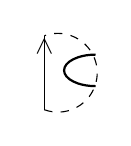
\begin{tikzpicture}[scale = 0.5, baseline = -3pt, rotate = 180]
\draw[dashed] (70:1) arc(70:290:1);
\draw (-70:1) -- (70:1) node[pos = 0.15,sloped]{\small $>$};
\draw[thick] (70:1)++ (-1.3,-0.6) arc(90:-90:0.8 and 0.4);
\end{tikzpicture} = q^{-\frac{1}{2}} 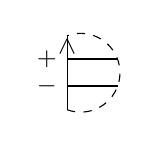
\begin{tikzpicture}[scale = 0.5, baseline = -3pt, rotate = 180]
\draw[dashed] (70:1) arc(70:290:1);
\draw (-70:1) -- (70:1) node[pos = 0.15,sloped]{\small $>$};
\draw[thick] (70:1)++ (0,-0.6) node[left]{\small $-$} -- ++(-1.3,0);
\draw[thick] (-70:1)++ (0,0.6) node[left]{\small $+$} -- ++(-1.3,0);
\end{tikzpicture} -q^{-\frac{5}{2}} 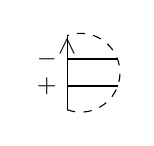
\begin{tikzpicture}[scale = 0.5, baseline = -3pt, rotate = 180]
\draw[dashed] (70:1) arc(70:290:1);
\draw (-70:1) -- (70:1) node[pos = 0.15,sloped]{\small $>$};
\draw[thick] (70:1)++ (0,-0.6) node[left]{\small $+$} -- ++(-1.3,0);
\draw[thick] (-70:1)++ (0,0.6) node[left]{\small $-$} -- ++(-1.3,0);
\end{tikzpicture}.
\]
\end{Proposition}

\begin{Remark}
It is easy to check that $\mathscr{S}(\mathfrak{S} \sqcup \mathfrak{S}') \simeq \mathscr{S}(\mathfrak{S}) \otimes_k \mathscr{S}(\mathfrak{S}')$ since all relations happen in a~connected disk.
\end{Remark}

\begin{Definition} [see {\cite[Section~3.1]{TTQLe}} for details]
Let $\mathfrak{S}$ be a marked surface and $c$ an ideal arc on~$\mathfrak{S}$, joining two marked points in $\overline{\mathfrak{S}}$. Denote by ${\rm Cut}_c(\mathfrak{S})$ the marked surface obtained by cutting $\mathfrak{S}$ along~$c$.

Given a stated tangle $\alpha$ on $\mathfrak{S}$, one can cut it along $c$ and get a tangle ${\rm Cut}_c(\alpha)$ on ${\rm Cut}_c(\mathfrak{S})$. This tangle has new boundary points, two lifts per points of $\alpha \cap c$, and we may give any state to these points. The obtained stated tangle is called a lift of $\alpha$ if the two lifts of a point of $\alpha \cap c$ have same state.
\end{Definition}

This definition is not perfectly innocent and it seems that one could have chosen different state-matching patterns for lifts, see Remark \ref{rmkChoiceCutting}.

\begin{Theorem}[{\cite[Theorem~3.1]{TTQLe}}]\label{splitmorph} Let $\mathfrak{S}$ be a marked surface and $c$ an ideal arc. The map $\rho_c\colon \mathscr{S}(\mathfrak{S}) \to \mathscr{S}({\rm Cut}_c(\mathfrak{S}))$, $\alpha \mapsto \sum_{\rm lifts} \tilde{\alpha}$ is well-defined $($it only depends on the isotopy class of~$\alpha)$ and is an injective algebra morphism. Moreover, the splitting morphisms $\rho_c$ and $\rho_{c'}$ associated to two disjoint ideal arcs $c$ and $c'$ commute.
\end{Theorem}

\begin{Example}
The bigon $B$ is the marked surface $(\mathbb{D},\{\pm i\})$, the disk with two marked points. The algebra $\mathscr{S}(B)$ is generated as an algebra by the
\[
{}_\mu\beta_\nu = 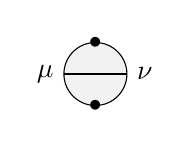
\begin{tikzpicture}[scale = 0.8, baseline = -5pt]
\fill [gray!10] (0,0) circle (0.5);
\draw (0,0) circle (0.5);
\node at (0,-0.5){\small $\bullet$};
\node at (0,0.5){\small $\bullet$};
\draw [thick] (-0.5,0) node[left]{$\mu$} -- (0.5,0) node[right]{$\nu$};
\end{tikzpicture}\!\!, \qquad
\mu,\nu \in \{\pm\},
\]
and has basis the
\[_{\vec{\mu}}\beta_{\vec{\nu}} = 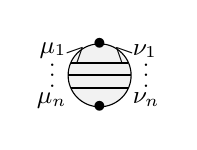
\begin{tikzpicture}[scale = 0.8, baseline = -5pt]
\fill [gray!10] (0,0) circle (0.5);
\draw (0,0) circle (0.5);
\node[rotate = 45] at (135:0.5) {\small $>$};
\node[rotate = -45] at (45:0.5) {\small $<$};
\node at (0,-0.5){\small $\bullet$};
\node at (0,0.5){\small $\bullet$};
\draw [thick] (-0.5,0) node[rotate = 90, above]{\footnotesize $\cdots$} -- (0.5,0) node[rotate = 90, below]{\footnotesize $\cdots$};
\draw [thick] (-0.45,-0.2) node[below left = -2pt]{\small $\mu_n$} -- (0.45,-0.2) node[below right = -2pt]{\small $\nu_n$};
\draw [thick] (-0.45,0.2) node[above left = -2pt]{\small $\mu_1$} -- (0.45,0.2) node[above right = -2pt]{\small $\nu_1$};
\end{tikzpicture}\!,
\]
where $\vec{\mu} = (\mu_1,\ldots,\mu_n)$ and $\vec{\nu} = (\nu_1,\ldots,\nu_n)$ are decreasing sequences of signs.

It is a bialgebra with coproduct given by cutting along the ``unique'' arc joining the two marked points \[
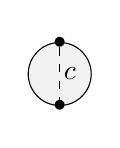
\begin{tikzpicture}[scale = 0.8, baseline = -5pt]
\fill [gray!10] (0,0) circle (0.5);
\draw (0,0) circle (0.5);
\node at (0,-0.5){\small $\bullet$};
\node at (0,0.5){\small $\bullet$};
\draw [dashed] (0,-0.5) -- (0,0.5) node[midway, right = -2pt]{$c$};
\end{tikzpicture}, \qquad
\Delta=\rho_c\colon\ \mathscr{S}(B) \to \mathscr{S}(B \sqcup B) \simeq \mathscr{S}(B) \otimes \mathscr{S}(B).
\]
Coassociativity comes from the second part of Theorem~\ref{splitmorph}. The counit $\varepsilon\colon \mathscr{S}(B) \to k$ is defined on the basis by $\varepsilon(_{\vec{\mu}}\beta_{\vec{\nu}}) = \delta_{\vec{\mu},\vec{\nu}}$.
It is a Hopf algebra with antipode
\[
S\Bigg(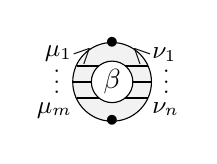
\begin{tikzpicture}[scale = 1, baseline = -5pt]
\fill [gray!10] (0,0) circle (0.5);
\draw (0,0) circle (0.5);
\node[rotate = 45] at (135:0.5) {\small $>$};
\node[rotate = -45] at (45:0.5) {\small $<$};
\node at (0,-0.5){\small $\bullet$};
\node at (0,0.5){\small $\bullet$};
\draw [thick] (-0.5,0) node[rotate = 90, above]{\footnotesize $\cdots$} -- (0.5,0) node[rotate = 90, below]{\footnotesize $\cdots$};
\draw [thick] (-0.45,-0.2) node[below left = -2pt]{\small $\mu_m$} -- (0.45,-0.2) node[below right = -2pt]{\small $\nu_n$};
\draw [thick] (-0.45,0.2) node[above left = -2pt]{\small $\mu_1$} -- (0.45,0.2) node[above right = -2pt]{\small $\nu_1$};
\node[circle, fill = white, draw = black, inner sep = 1.5pt] at (0,0) {$\beta$};
\end{tikzpicture}\!\!\Bigg)=
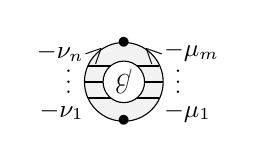
\begin{tikzpicture}[scale = 1, baseline = -5pt]
\fill [gray!10] (0,0) circle (0.5);
\draw (0,0) circle (0.5);
\node[rotate = 45] at (135:0.5) {\small $>$};
\node[rotate = -45] at (45:0.5) {\small $<$};
\node at (0,-0.5){\small $\bullet$};
\node at (0,0.5){\small $\bullet$};
\draw [thick] (-0.5,0) node[rotate = 90, above]{\footnotesize $\cdots$} -- (0.5,0) node[rotate = 90, below]{\footnotesize $\cdots$};
\draw [thick] (-0.45,-0.2) node[below left = -2pt]{\small $-\nu_1$} -- (0.45,-0.2) node[below right = -2pt]{\small $-\mu_1$};
\draw [thick] (-0.45,0.2) node[above left = -2pt]{\small $-\nu_n$} -- (0.45,0.2) node[above right = -2pt]{\small $-\mu_m$};
\node[circle, rotate = 180, fill = white, draw = black, inner sep = 1.5pt] at (0,0) {$\beta$};
\end{tikzpicture}
 .\ \frac{C(\vec{\nu})}{C(\vec{\mu})},\qquad
\text{where}\qquad C(\vec{\nu}):= \prod_{i=1}^n C(\nu_i).
 \]
It is coquasitriangular with co-$R$-matrix
\[
R(\alpha \otimes \beta) =\varepsilon
\raisebox{0pt}{$\left(\rule{-3pt}{22pt}\right.$}\!
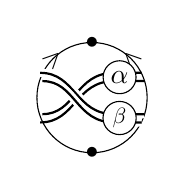
\begin{tikzpicture}[scale = 0.7, baseline = 0pt, rotate = 180]
\draw (0,-1) node{\small $\bullet$} arc(-90:90:1) node[near start, sloped]{\small $>$} node{\small $\bullet$};
\draw (0,-1) arc(-90:-270:1) node[near start, sloped]{\small $<$};
\draw[thick] (-0.9,-0.45) -- (-0.4,-0.45) .. controls (0.3,-0.45) and (0.3,0.3).. (0.9,0.3);
\draw[thick] (-0.94,-0.3) -- (-0.4,-0.3) .. controls (0.3,-0.3) and (0.3,0.45).. (0.94,0.45);
\draw[line width = 3pt, white] (-0.94,0.3) -- (-0.4,0.3) .. controls (0.3,0.3) and (0.3,-0.45).. (0.94,-0.45);
\draw[thick] (-0.94,0.3) -- (-0.4,0.3) .. controls (0.3,0.3) and (0.3,-0.45).. (0.94,-0.45);
\draw[line width = 3pt, white] (-0.9,0.45) -- (-0.4,0.45) .. controls (0.3,0.45) and (0.3,-0.3).. (0.9,-0.3);
\draw[thick] (-0.9,0.45) -- (-0.4,0.45) .. controls (0.3,0.45) and (0.3,-0.3).. (0.9,-0.3);
\node[circle, fill=white, draw = black, scale = 0.8, inner sep = 1.5pt] (X) at (-0.5,0.37){$\beta$};
\node[circle, fill=white, draw = black, scale = 1, inner sep = 1.5pt] (X) at (-0.5,-0.37){$\alpha$};
\end{tikzpicture}\!
\raisebox{0pt}{$\left.\rule{-3pt}{22pt}\right)$}\!,
\]
see \cite[Theorem~3.5]{Cos}.
It is coribbon with coribbon functional
\[
\theta(\alpha) = \varepsilon
\raisebox{0pt}{$\left(\rule{-3pt}{22pt}\right.$}\!
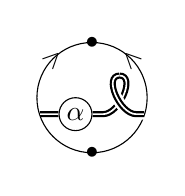
\begin{tikzpicture}[scale = 0.7, baseline = 0pt]
\draw (0,-1) node{\small $\bullet$} arc(-90:90:1) node[near end, sloped]{\small $<$} node{\small $\bullet$};
\draw (0,-1) arc(-90:-270:1) node[near end, sloped]{\small $>$};
\node[circle, draw = black, scale = 1, inner sep = 1.5pt] (X) at (-0.3,-0.3){$\alpha$};
\draw[thick, double] (-0.94,-0.3) -- (X) -- (0.2,-0.3) .. controls (0.5,-0.3) and (0.8,0.4).. (0.5,0.4);
\draw[line width = 4pt, white] (0.5,0.4).. controls (0.2,0.4) and (0.5,-0.3) .. (0.8,-0.3) -- (0.94,-0.3);
\draw[thick, double] (0.5,0.4).. controls (0.2,0.4) and (0.5,-0.3) .. (0.8,-0.3) -- (0.94,-0.3);
\end{tikzpicture}\!
\raisebox{0pt}{$\left.\rule{-3pt}{22pt}\right)$}\!.
\]
\end{Example}

\begin{Proposition}[{\cite[Theorem~4.1]{TTQLe}, \cite[Section~2.2]{KorQue}}, {\cite[Theorem~3.4]{Cos}}]
One has an isomorphism of coribbon Hopf algebras $\mathscr{S}(B)\simeq \Oq$ given on the generators by $_+\beta_+\mapsto a$, ${}_-\beta_{-}\mapsto d$,  ${}_+\beta_{-}\mapsto b$ and ${}_-\beta_{+}\mapsto c$.
\end{Proposition}
Stated skein algebras provide great examples of (possibly infinite-dimensional) $\Oq$ or $\mathscr{S}(B)$-comodules.

Given a marked surface $\mathfrak{S}$ and a boundary edge $e$ of $\mathfrak{S}$, we can consider an ideal arc $c$ going along~$e$ but inside $\mathring{\mathfrak{S}}$. The piece between $e$ and $c$ is a bigon, and the rest is homeomorphic to the original surface. The splitting morphism along $c$, $\Delta = \rho_c\colon \mathscr{S}(\mathfrak{S}) \to \mathscr{S}(\mathfrak{S}\sqcup B)\simeq \mathscr{S}(\mathfrak{S})\otimes \mathscr{S}(B)$ endows $\mathscr{S}(\mathfrak{S})$ with right $\Oq$-comodule structure.
$$
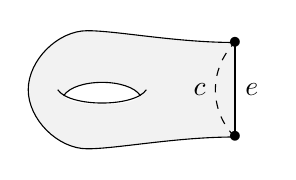
\begin{tikzpicture}[xscale = 0.75, yscale = 0.75,baseline = 10pt]
\fill[gray!10] (3.5,0.2) coordinate (B)	.. controls (2.5,0.2) and (1.5,0 ) .. (1,0)	.. controls (0.5,0 ) and (0,0.5 ) .. (0,1)	.. controls (0,1.5 ) and (0.5,2 ) .. (1,2)	.. controls (1.5,2 ) and (2.5,1.8) .. (3.5,1.8) coordinate (H) -- cycle ;
\fill[white] (0.6,0.9) .. controls (0.7,0.7) and (1.8,0.7) .. (1.9,0.9) .. controls (1.7,1.2) and (0.8,1.2) .. (0.6,0.9);
\draw (0.5,1) .. controls (0.7,0.7) and (1.8,0.7) .. (2,1);
\draw (0.6,0.9) .. controls (0.8,1.2) and (1.7,1.2) .. (1.9,0.9);
\draw (3.5,0.2) node{\small $\bullet$}	.. controls (2.5,0.2) and (1.5,0 ) .. (1,0)	.. controls (0.5,0 ) and (0,0.5 ) .. (0,1)	.. controls (0,1.5 ) and (0.5,2 ) .. (1,2)	.. controls (1.5,2 ) and (2.5,1.8) .. (3.5,1.8) node{\small $\bullet$};
\draw[thick] (B) -- (H) node[midway,right]{$e$};
\path[dashed, bend left = 150pt, in = 135, out = 45] (B) edge node[midway,left]{$c$} (H);
\end{tikzpicture}
$$
It is compatible with its algebra structure, namely $\mathscr{S}(\mathfrak{S})$ is an $\Oq$-comodule-algebra, see \cite[Proposition~4.1]{Cos}.

\begin{Definition}
Let $\operatorname{rot}\colon B \to B$ be the homeomorphism of marked surfaces given by the planar 180 degree rotation. It induces $\operatorname{rot}_*\colon \mathscr{S}(B) \to \mathscr{S}(B)$, with
\[
\operatorname{rot}_*\Bigg(
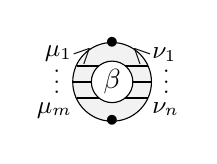
\begin{tikzpicture}[scale = 1, baseline = -5pt]
\fill [gray!10] (0,0) circle (0.5);
\draw (0,0) circle (0.5);
\node[rotate = 45] at (135:0.5) {\small $>$};
\node[rotate = -45] at (45:0.5) {\small $<$};
\node at (0,-0.5){\small $\bullet$};
\node at (0,0.5){\small $\bullet$};
\draw [thick] (-0.5,0) node[rotate = 90, above]{\footnotesize $\cdots$} -- (0.5,0) node[rotate = 90, below]{\footnotesize $\cdots$};
\draw [thick] (-0.45,-0.2) node[below left = -2pt]{\small $\mu_m$} -- (0.45,-0.2) node[below right = -2pt]{\small $\nu_n$};
\draw [thick] (-0.45,0.2) node[above left = -2pt]{\small $\mu_1$} -- (0.45,0.2) node[above right = -2pt]{\small $\nu_1$};
\node[circle, fill = white, draw = black, inner sep = 1.5pt] at (0,0) {$\beta$};
\end{tikzpicture}
\Bigg) =
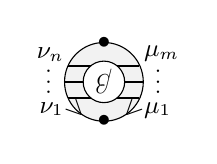
\begin{tikzpicture}[scale = 1, baseline = -5pt]
\fill [gray!10] (0,0) circle (0.5);
\draw (0,0) circle (0.5);
\node[rotate = 135] at (-135:0.5) {\small $<$};
\node[rotate = -135] at (-45:0.5) {\small $>$};
\node at (0,-0.5){\small $\bullet$};
\node at (0,0.5){\small $\bullet$};
\draw [thick] (-0.5,0) node[rotate = 90, above]{\footnotesize $\cdots$} -- (0.5,0) node[rotate = 90, below]{\footnotesize $\cdots$};
\draw [thick] (-0.45,-0.2) node[below left = -2pt]{\small $\nu_1$} -- (0.45,-0.2) node[below right = -2pt]{\small $\mu_1$};
\draw [thick] (-0.45,0.2) node[above left = -2pt]{\small $\nu_n$} -- (0.45,0.2) node[above right = -2pt]{\small $\mu_m$};
\node[circle, rotate = 180, fill = white, draw = black, inner sep = 1.5pt] at (0,0) {$\beta$};
\end{tikzpicture}
\]
which is an algebra isomorphism. It reverses the coproduct, namely
\[
\Delta\circ \operatorname{rot}_*(\beta) =
 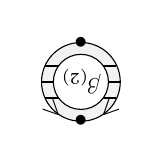
\begin{tikzpicture}[scale = 1, baseline = -5pt]
\fill [gray!10] (0,0) circle (0.5);
\draw (0,0) circle (0.5);
\node[rotate = 135] at (-135:0.5) {\small $<$};
\node[rotate = -135] at (-45:0.5) {\small $>$};
\node at (0,-0.5){\small $\bullet$};
\node at (0,0.5){\small $\bullet$};
\draw [thick] (-0.5,0) -- (0.5,0);
\draw [thick] (-0.45,-0.2) -- (0.45,-0.2) ;
\draw [thick] (-0.45,0.2) -- (0.45,0.2);
\node[circle, rotate = 180, fill = white, draw = black, inner sep = 1pt] at (0,0) {\footnotesize $\beta_{(2)}$};
\end{tikzpicture} \otimes 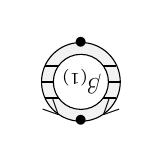
\begin{tikzpicture}[scale = 1, baseline = -5pt]
\fill [gray!10] (0,0) circle (0.5);
\draw (0,0) circle (0.5);
\node[rotate = 135] at (-135:0.5) {\small $<$};
\node[rotate = -135] at (-45:0.5) {\small $>$};
\node at (0,-0.5){\small $\bullet$};
\node at (0,0.5){\small $\bullet$};
\draw [thick] (-0.5,0) -- (0.5,0);
\draw [thick] (-0.45,-0.2) -- (0.45,-0.2) ;
\draw [thick] (-0.45,0.2) -- (0.45,0.2);
\node[circle, rotate = 180, fill = white, draw = black, inner sep = 1pt] at (0,0) {\footnotesize $\beta_{(1)}$};
\end{tikzpicture} = (\operatorname{rot}_*\otimes \operatorname{rot}_*) \circ \Delta^{\rm op} (\beta),
\]
and preserves the counit, because $\varepsilon(\operatorname{rot}_*(_{\vec{\mu}}\beta_{\vec{\nu}})) = \varepsilon(_{\vec{\nu}}\beta_{\vec{\mu}}) = \delta_{\vec{\nu},\vec{\mu}} = \delta_{\vec{\mu},\vec{\nu}}$.
On $\Oq$, it is given by $r\left(\begin{smallmatrix}a&b\\c&d\end{smallmatrix}\right) = \left( \begin{smallmatrix}a&c\\b&d\end{smallmatrix}\right)$.
\end{Definition}

\begin{Remark}If one sees the edge $e$ at the left instead of the right of the surface, one gets a~structure of left $\Oq$-comodule. One can easily get from one to another by rotating the whole picture. Namely, the left coaction $\Delta_{\rm l}$ is obtained from the right coaction $\Delta_{\rm r}$ by rotating the bigon by 180 degrees. In \cite[Proposition~4.1]{Cos} one gets $\Delta_{\rm l} = \operatorname{fl} \circ ({\rm Id}_{\mathscr{S}(\mathfrak{S})} \otimes \operatorname{rot}_*) \circ \Delta_{\rm r}$, where $\operatorname{fl}$ denotes the flip of tensors.
$$
\begin{tikzpicture}[xscale = 0.75, yscale = 0.5,baseline = 10pt]
\fill[gray!10] (3.5,0.2) coordinate (B)	.. controls (2.5,0.2) and (1.5,0 ) .. (1,0)	.. controls (0.5,0 ) and (0,0.5 ) .. (0,1)	.. controls (0,1.5 ) and (0.5,2 ) .. (1,2)	.. controls (1.5,2 ) and (2.5,1.8) .. (3.5,1.8) coordinate (H) to[bend right = 150pt, in = -135, out = -45] (B) ;
\fill[white] (0.6,0.9) .. controls (0.7,0.7) and (1.8,0.7) .. (1.9,0.9) .. controls (1.7,1.2) and (0.8,1.2) .. (0.6,0.9);
\draw (0.5,1) .. controls (0.7,0.7) and (1.8,0.7) .. (2,1);
\draw (0.6,0.9) .. controls (0.8,1.2) and (1.7,1.2) .. (1.9,0.9);
\draw (3.5,0.2)node{\small $\bullet$}	.. controls (2.5,0.2) and (1.5,0 ) .. (1,0)	.. controls (0.5,0 ) and (0,0.5 ) .. (0,1)	.. controls (0,1.5 ) and (0.5,2 ) .. (1,2)	.. controls (1.5,2 ) and (2.5,1.8) .. (3.5,1.8) node{\small $\bullet$};
\path[dashed, bend left = 150pt, in = 135, out = 45] (B) edge node[midway,left]{$c$} (H);
\node [right= 8pt of B, inner sep = 0pt] (B') {};
\node [right= 8pt of H, inner sep = 0pt] (H') {};
\fill[gray!10] (B'.center)to[bend left = 150pt, in = 135, out = 45] (H'.center) to[bend left = 150pt, in = 135, out = 45] (B');
\draw[dashed] (B'.center) to[bend left = 150pt, in = 135, out = 45] node[pos = 0]{\small $\bullet$} node[pos = 1]{\small $\bullet$} node[midway]{\small $W$} (H'.center);
\draw[dashed] (H'.center) to[bend left = 150pt, in = 135, out = 45] node[midway]{\small $E$} node[pos = 1,below]{\small $S$} node[pos = 0,above]{\small $N$} (B'.center);
\draw[->] (0,0) to[bend right] ++(0,-1.5);
\begin{scope}[xshift = 4.5cm, yshift = -2cm, rotate = 180]
\fill[gray!10] (3.5,0.2) coordinate (B)	.. controls (2.5,0.2) and (1.5,0 ) .. (1,0)	.. controls (0.5,0 ) and (0,0.5 ) .. (0,1)	.. controls (0,1.5 ) and (0.5,2 ) .. (1,2)	.. controls (1.5,2 ) and (2.5,1.8) .. (3.5,1.8) coordinate (H) to[bend right = 150pt, in = -135, out = -45] (B) ;
\fill[white] (0.6,0.9) .. controls (0.7,0.7) and (1.8,0.7) .. (1.9,0.9) .. controls (1.7,1.2) and (0.8,1.2) .. (0.6,0.9);
\draw (0.5,1) .. controls (0.7,0.7) and (1.8,0.7) .. (2,1);
\draw (0.6,0.9) .. controls (0.8,1.2) and (1.7,1.2) .. (1.9,0.9);
\draw (3.5,0.2)node{\small $\bullet$}	.. controls (2.5,0.2) and (1.5,0 ) .. (1,0)	.. controls (0.5,0 ) and (0,0.5 ) .. (0,1)	.. controls (0,1.5 ) and (0.5,2 ) .. (1,2)	.. controls (1.5,2 ) and (2.5,1.8) .. (3.5,1.8) node{\small $\bullet$};
\path[dashed, bend left = 150pt, in = 135, out = 45] (B) edge node[midway,right]{$c$} (H);
\node [left= 8pt of B, inner sep = 0pt] (B') {};
\node [left= 8pt of H, inner sep = 0pt] (H') {};
\fill[gray!10] (B'.center)to[bend left = 150pt, in = 135, out = 45] (H'.center) to[bend left = 150pt, in = 135, out = 45] (B');
\draw[dashed] (B'.center) to[bend left = 150pt, in = 135, out = 45] node[pos = 0]{\small $\bullet$} node[pos = 1]{\small $\bullet$} node[midway]{\small $W$} (H'.center);
\draw[dashed] (H'.center) to[bend left = 150pt, in = 135, out = 45] node[midway]{\small $E$} node[pos = 1,above]{\small $S$} node[pos = 0,below]{\small $N$} (B'.center);
\draw[->] (0,0) to[bend right] ++(0,-1.5);
\end{scope}
\end{tikzpicture}
$$
Actually, one gets such a structure for each boundary edge of $\mathfrak{S}$, and if $\mathfrak{S}$ has $n$ right boundary edges and $m$ left, $\mathscr{S}(\mathfrak{S})$ is an $\big(\Oq^{\otimes n},\Oq^{\otimes m}\big)$-bicomodule algebra.
\end{Remark}

\begin{Remark}\label{rmkFormActOnSS}
The structure forms on $\mathscr{S}(B)$, such as the co-$R$-matrix or the coribbon functional, are often defined using the counit on some transformation of the tangle. This has a direct interpretation on how this form then acts on comodules.

Let $\varphi\colon\mathscr{S}(B) \to k$ be given by some
\[
\varphi\raisebox{-3pt}{$\left(\rule{0pt}{22pt}\right.$}\!\!
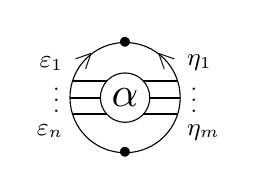
\begin{tikzpicture}[scale = 0.7, baseline = 0pt]
\draw (0,-1) node{\small $\bullet$} arc(-90:90:1) node[near end, sloped]{\small $<$} node{\small $\bullet$};
\draw (0,-1) arc(-90:-270:1) node[near end, sloped]{\small $>$};
\draw[thick] (-0.94,-0.3)node[below left]{\small $\varepsilon_n$} -- (0.94,-0.3)node[below right]{\small $\eta_m$};
\draw[thick] (-1,0) node[yshift=2pt,left]{\footnotesize $\vdots$} -- (1,0)node[yshift=2pt,right]{\footnotesize $\vdots$};
\draw[thick] (-0.94,0.3) node[above left]{\small $\varepsilon_1$} -- (0.94,0.3)node[above right]{\small $\eta_1$};
\node[circle, fill=white, draw = black, scale = 1.5, inner sep = 1.5pt] (X) at (0,0){$\alpha$};
\end{tikzpicture}\!\!
\raisebox{-3pt}{$\left.\rule{0pt}{22pt}\right)$}
 = \varepsilon
\raisebox{-3pt}{$\left(\rule{0pt}{32pt}\right.$}\!\!\!
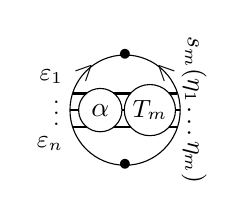
\begin{tikzpicture}[scale = 0.7, baseline = 0pt]
\draw (0,-1) node{\small $\bullet$} arc(-90:90:1) node[near end, sloped]{\small $<$} node{\small $\bullet$};
\draw (0,-1) arc(-90:-270:1) node[near end, sloped]{\small $>$};
\draw[thick] (-0.94,-0.3)node[below left]{\small $\varepsilon_n$} -- (0.94,-0.3);
\draw[thick] (-1,0) node[yshift=2pt,left]{\footnotesize $\vdots$} -- (1,0)node[xshift = 5pt, yshift = 0pt, rotate = -90]{\small $s_m(\eta_1 \dots \eta_m)$};
\draw[thick] (-0.94,0.3) node[above left]{\small $\varepsilon_1$} -- (0.94,0.3);
\node[circle, minimum width=0.55cm, fill=white, draw = black, scale = 1, inner sep = 1.5pt] (X) at (-0.45,0){$\alpha$};
\node[circle, minimum width=0.5cm,fill=white, draw = black, scale = 1, inner sep = 1.5pt] at (0.45,0){\small $T_m$};
\end{tikzpicture}\!
\raisebox{-3pt}{$\left.\rule{0pt}{32pt}\right)$},
\]
where $T_m,\ m \in \mathbb{N},$ is a family of tangles with $m$ right and $m$ left boundary points and $s_m\colon \{\pm\}^m\to {\rm vect}_ k(\{\pm\}^m)$. Here, we allowed $s_m$ to have values in formal linear combination of $m$-tuples of states because in the definition of the co-$R$-matrix for example one needs coefficients depending on the states. What we mean by a tangle $\alpha$ with state a formal linear combination of states $\sum_i \lambda_i \vec{\eta}_i$ is the linear sum of stated tangles $\alpha_{\sum_i \lambda_i \vec{\eta}_i} := \sum_i \lambda_i \alpha_{\vec{\eta}_i}$.
Note that the $T_m$'s and the $s_m$'s should satisfy extra conditions for this to be well-defined on $\mathscr{S}(B)$. Then for a marked surface $\mathfrak{S}$ with a right edge $e$, the map $\Phi_{\mathscr{S}(\mathfrak{S})}\colon \mathscr{S}(\mathfrak{S}) \overset{\Delta}{\to} \mathscr{S}(\mathfrak{S}) \otimes \mathscr{S}(B) \overset{{\rm Id} \otimes \varphi}{\longrightarrow} \mathscr{S}(\mathfrak{S})$ is given by
\[
\begin{array}{ll}
\begin{tikzpicture}[scale = 0.7, baseline = 0pt]
\draw (0,-1) node{\small $\bullet$} arc(-90:90:1) node[near end, sloped]{\small $<$} node{\small $\bullet$};
\draw (0,-1) -- (-1,-1);
\draw (0,1) -- (-1,1);
\draw[thick] (-1,-0.3) -- (0.94,-0.3)node[below right]{\small $\eta_m$};
\draw[thick] (-1,0) -- (1,0)node[yshift=2pt,right]{\footnotesize $\vdots$};
\draw[thick] (-1,0.3) -- (0.94,0.3)node[above right]{\small $\eta_1$};
\node[fill=white, minimum width = 1cm, minimum height = 0.7cm, leftymissy, inner sep = 1.5pt] (X) at (-0.5,0){$\alpha$};
\end{tikzpicture}
&\overset{\Delta}{\longmapsto} \sum_{\vec{\nu}}
\raisebox{-3pt}{$\left(\rule{0pt}{26pt}\right.$}
\begin{tikzpicture}[scale = 0.7, baseline = 0pt]
\draw (0,-1) node{\small $\bullet$} arc(-90:90:1) node[near end, sloped]{\small $<$} node{\small $\bullet$};
\draw (0,-1) -- (-1,-1);
\draw (0,1) -- (-1,1);
\draw[thick] (-1,-0.3) -- (0.94,-0.3)node[below right]{\small $\nu_m$};
\draw[thick] (-1,0) -- (1,0)node[yshift=2pt,right]{\footnotesize $\vdots$};
\draw[thick] (-1,0.3) -- (0.94,0.3)node[above right]{\small $\nu_1$};
\node[fill=white, minimum width = 1cm, minimum height = 0.7cm, leftymissy, inner sep = 1.5pt] (X) at (-0.5,0){$\alpha$};
\end{tikzpicture} \otimes
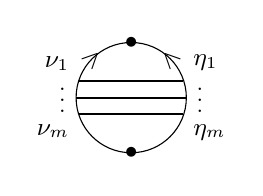
\begin{tikzpicture}[scale = 0.7, baseline = 0pt]
\draw (0,-1) node{\small $\bullet$} arc(-90:90:1) node[near end, sloped]{\small $<$} node{\small $\bullet$};
\draw (0,-1) arc(-90:-270:1) node[near end, sloped]{\small $>$};
\draw[thick] (-0.94,-0.3)node[below left]{\small $\nu_m$} -- (0.94,-0.3)node[below right]{\small $\eta_m$};
\draw[thick] (-1,0) node[yshift=2pt,left]{\footnotesize $\vdots$} -- (1,0)node[yshift=2pt,right]{\footnotesize $\vdots$};
\draw[thick] (-0.94,0.3) node[above left]{\small $\nu_1$} -- (0.94,0.3)node[above right]{\small $\eta_1$};
\end{tikzpicture}\!\!\!
\raisebox{-3pt}{$\left.\rule{0pt}{26pt}\right)$}
\\
& \overset{{\rm Id}\otimes \varphi}{\longmapsto} ({\rm Id} \otimes \varepsilon)
\raisebox{-3pt}{$\left(\rule{0pt}{32pt}\right.$}
\begin{tikzpicture}[scale = 0.7, baseline = 0pt]
\draw (0,-1) node{\small $\bullet$} arc(-90:90:1) node[near end, sloped]{\small $<$} node{\small $\bullet$};
\draw (0,-1) -- (-1,-1);
\draw (0,1) -- (-1,1);
\draw[thick] (-1,-0.3) -- (0.94,-0.3)node[below right]{\small $\nu_m$};
\draw[thick] (-1,0) -- (1,0)node[yshift=2pt,right]{\footnotesize $\vdots$};
\draw[thick] (-1,0.3) -- (0.94,0.3)node[above right]{\small $\nu_1$};
\node[fill=white, minimum width = 1cm, minimum height = 0.7cm, leftymissy, inner sep = 1.5pt] (X) at (-0.5,0){$\alpha$};
\end{tikzpicture} \otimes
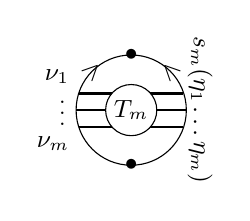
\begin{tikzpicture}[scale = 0.7, baseline = 0pt]
\draw (0,-1) node{\small $\bullet$} arc(-90:90:1) node[near end, sloped]{\small $<$} node{\small $\bullet$};
\draw (0,-1) arc(-90:-270:1) node[near end, sloped]{\small $>$};
\draw[thick] (-0.94,-0.3)node[below left]{\small $\nu_m$} -- (0.94,-0.3);
\draw[thick] (-1,0) node[yshift=2pt,left]{\footnotesize $\vdots$} -- (1,0)node[xshift = 5pt, yshift = 0pt, rotate = -90]{\small $s_m(\eta_1 \dots \eta_m)$};
\draw[thick] (-0.94,0.3) node[above left]{\small $\nu_1$} -- (0.94,0.3);
\node[circle, minimum width=0.5cm,fill=white, draw = black, scale = 1, inner sep = 1.5pt] at (0,0){\small $T_m$};
\end{tikzpicture}
\raisebox{-3pt}{$\left.\rule{0pt}{32pt}\right)$}
\\
& \overset{\rm splitting}{\underset{\rm well\ def}{=}} ({\rm Id} \otimes \varepsilon)
\raisebox{-3pt}{$\left(\rule{0pt}{32pt}\right.$}
\begin{tikzpicture}[scale = 0.7, baseline = 0pt]
\draw (0,-1) node{\small $\bullet$} arc(-90:90:1) node[near end, sloped]{\small $<$} node{\small $\bullet$};
\draw (0,-1) -- (-1,-1);
\draw (0,1) -- (-1,1);
\draw[thick] (-1,-0.3) -- (0.94,-0.3)node[below right]{\small $\nu_m$};
\draw[thick] (-1,0) -- (1,0)node[yshift=2pt,right]{\footnotesize $\vdots$};
\draw[thick] (-1,0.3) -- (0.94,0.3)node[above right]{\small $\nu_1$};
\node[fill=white, minimum width = 0.7cm, minimum height = 0.7cm, leftymissy, inner sep = 1.5pt] (X) at (-0.65,0){$\alpha$};
\node[circle, minimum width=0.5cm,fill=white, draw = black, scale = 1, inner sep = 1.5pt] at (0.4,0){\small $T_m$};
\end{tikzpicture} \otimes
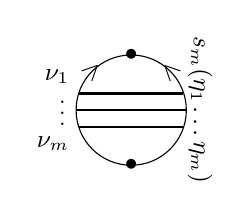
\begin{tikzpicture}[scale = 0.7, baseline = 0pt]
\draw (0,-1) node{\small $\bullet$} arc(-90:90:1) node[near end, sloped]{\small $<$} node{\small $\bullet$};
\draw (0,-1) arc(-90:-270:1) node[near end, sloped]{\small $>$};
\draw[thick] (-0.94,-0.3)node[below left]{\small $\nu_m$} -- (0.94,-0.3);
\draw[thick] (-1,0) node[yshift=2pt,left]{\footnotesize $\vdots$} -- (1,0)node[xshift = 5pt, yshift = 0pt, rotate = -90]{\small $s_m(\eta_1 \dots \eta_m)$};
\draw[thick] (-0.94,0.3) node[above left]{\small $\nu_1$} -- (0.94,0.3);
\end{tikzpicture}
\raisebox{-3pt}{$\left.\rule{0pt}{32pt}\right)$}
\overset{\rm counit}{=}
\begin{tikzpicture}[scale = 0.7, baseline = 0pt]
\draw (0,-1) node{\small $\bullet$} arc(-90:90:1) node[near end, sloped]{\small $<$} node{\small $\bullet$};
\draw (0,-1) -- (-1,-1);
\draw (0,1) -- (-1,1);
\draw[thick] (-1,-0.3) -- (0.94,-0.3);
\draw[thick] (-1,0) -- (1,0)node[xshift = 5pt, yshift = 0pt, rotate = -90]{\small $s_m(\eta_1 \dots \eta_m)$};
\draw[thick] (-1,0.3) -- (0.94,0.3);
\node[fill=white, minimum width = 0.7cm, minimum height = 0.7cm, leftymissy, inner sep = 1.5pt] (X) at (-0.65,0){$\alpha$};
\node[circle, minimum width=0.5cm,fill=white, draw = black, scale = 1, inner sep = 1.5pt] at (0.4,0){\small $T_m$};
\end{tikzpicture}.
\end{array}
\]
The co-$R$-matrix isn't exactly of this form, but the same kind of computation applies. Remember that the braiding on $\mathscr{S}(\mathfrak{S}) \otimes \mathscr{S}(\mathfrak{S})$ is defined using the coaction on each $\mathscr{S}(\mathfrak{S})$, the co-$R$-matrix on the $\mathscr{S}(B)^{\otimes 2}$ part thus obtained, and then flipping the two factors, namely $c_{\mathscr{S}(\mathfrak{S}),\mathscr{S}(\mathfrak{S})} = \operatorname{fl} \circ R_{24}\circ \big(\Delta_{\mathscr{S}(\mathfrak{S})}\otimes \Delta_{\mathscr{S}(\mathfrak{S})}\big)$. The braided opposite product on $\mathscr{S}(\mathfrak{S})$ is defined as $m^{\rm bop} := m \circ c_{\mathscr{S}(\mathfrak{S}),\mathscr{S}(\mathfrak{S})}$ and it has a nice geometric depiction, namely:
\[
\begin{array}{ll}
m^{\rm bop}(\alpha \otimes \beta) & = m \circ \operatorname{fl}
\raisebox{-3pt}{$\left(\rule{0pt}{26pt}\right.$}
\begin{tikzpicture}[scale = 0.7, baseline = 0pt]
\draw (0,-1) node{\small $\bullet$} arc(-90:90:1) node[near end, sloped]{\small $<$} node{\small $\bullet$};
\draw (0,-1) -- (-1,-1);
\draw (0,1) -- (-1,1);
\draw[thick] (-1,-0.3) -- (0.94,-0.3)node[below right]{\small $\nu_n$};
\draw[thick] (-1,0) -- (1,0)node[yshift=2pt,right]{\footnotesize $\vdots$};
\draw[thick] (-1,0.3) -- (0.94,0.3)node[above right]{\small $\nu_1$};
\node[fill=white, minimum width = 1cm, minimum height = 0.7cm, leftymissy, inner sep = 1.5pt] (X) at (-0.5,0){$\alpha_{(1)}$};
\end{tikzpicture} \otimes \begin{tikzpicture}[scale = 0.7, baseline = 0pt]
\draw (0,-1) node{\small $\bullet$} arc(-90:90:1) node[near end, sloped]{\small $<$} node{\small $\bullet$};
\draw (0,-1) -- (-1,-1);
\draw (0,1) -- (-1,1);
\draw[thick] (-1,-0.3) -- (0.94,-0.3)node[below right]{\small $\mu_m$};
\draw[thick] (-1,0) -- (1,0)node[yshift=2pt,right]{\footnotesize $\vdots$};
\draw[thick] (-1,0.3) -- (0.94,0.3)node[above right]{\small $\mu_1$};
\node[fill=white, minimum width = 1cm, minimum height = 0.7cm, leftymissy, inner sep = 1.5pt] (X) at (-0.5,0){$\beta_{(1)}$};
\end{tikzpicture}
\!.\
\varepsilon \raisebox{-3pt}{$\left(\rule{0pt}{26pt}\right.$}\!\!
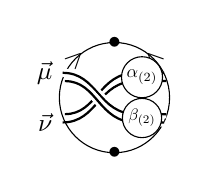
\begin{tikzpicture}[scale = 0.7, baseline = 0pt, rotate = 180]
\draw (0,-1) node{\small $\bullet$} arc(-90:90:1) node[near start, sloped]{\small $>$} node{\small $\bullet$};
\draw (0,-1) arc(-90:-270:1) node[near start, sloped]{\small $<$};
\draw[thick] (-0.9,-0.45) -- (-0.4,-0.45) .. controls (0.3,-0.45) and (0.3,0.3).. (0.9,0.3);
\draw[thick] (-0.94,-0.3) -- (-0.4,-0.3) .. controls (0.3,-0.3) and (0.3,0.45).. (0.94,0.45)node[left]{\small $\vec{\nu}$};
\draw[line width = 3pt, white] (-0.94,0.3) -- (-0.4,0.3) .. controls (0.3,0.3) and (0.3,-0.45).. (0.94,-0.45);
\draw[thick] (-0.94,0.3) -- (-0.4,0.3) .. controls (0.3,0.3) and (0.3,-0.45).. (0.94,-0.45)node[left]{\small $\vec{\mu}$};
\draw[line width = 3pt, white] (-0.9,0.45) -- (-0.4,0.45) .. controls (0.3,0.45) and (0.3,-0.3).. (0.9,-0.3);
\draw[thick] (-0.9,0.45) -- (-0.4,0.45) .. controls (0.3,0.45) and (0.3,-0.3).. (0.9,-0.3);
\node[circle, fill=white, draw = black, scale = 0.6, inner sep = 1.5pt] (X) at (-0.5,0.37){$\beta_{(2)}$};
\node[circle, fill=white, draw = black, scale = 0.65, inner sep = 1.5pt] (X) at (-0.5,-0.37){$\alpha_{(2)}$};
\end{tikzpicture}\!\!
\raisebox{-3pt}{$\left.\rule{0pt}{26pt}\right)$}\!\raisebox{-3pt}{$\left.\rule{0pt}{26pt}\right)$}
\\
&=
 \begin{tikzpicture}[scale = 0.7, baseline = 0pt]
\draw (0,-1) node{\small $\bullet$} arc(-90:90:1) node[near end, sloped]{\small $<$} node{\small $\bullet$};
\draw (0,-1) -- (-1,-1);
\draw (0,1) -- (-1,1);
\draw[thick, double] (-1,-0.3) -- (0.94,-0.3)node[right=-2pt]{\small $\vec{\nu}$};
\draw[thick, double] (-1,0.3) -- (0.94,0.3)node[right=-2pt]{\small $\vec{\mu}$};
\node[scale = 0.8, fill=white, minimum width = 1cm, minimum height = 0.5cm, leftymissy, inner sep = 1.5pt] (X) at (-0.5,0.35){\small $\beta_{(1)}$};
\node[scale = 0.8, fill=white, minimum width = 1cm, minimum height = 0.5cm, leftymissy, inner sep = 1.5pt] (X) at (-0.5,-0.35){\small $\alpha_{(1)}$};
\end{tikzpicture}
.\
\varepsilon \raisebox{-3pt}{$\left(\rule{0pt}{26pt}\right.$}\!\!
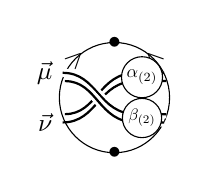
\begin{tikzpicture}[scale = 0.7, baseline = 0pt, rotate = 180]
\draw (0,-1) node{\small $\bullet$} arc(-90:90:1) node[near start, sloped]{\small $>$} node{\small $\bullet$};
\draw (0,-1) arc(-90:-270:1) node[near start, sloped]{\small $<$};
\draw[thick] (-0.9,-0.45) -- (-0.4,-0.45) .. controls (0.3,-0.45) and (0.3,0.3).. (0.9,0.3);
\draw[thick] (-0.94,-0.3) -- (-0.4,-0.3) .. controls (0.3,-0.3) and (0.3,0.45).. (0.94,0.45)node[left]{\small $\vec{\nu}$};
\draw[line width = 3pt, white] (-0.94,0.3) -- (-0.4,0.3) .. controls (0.3,0.3) and (0.3,-0.45).. (0.94,-0.45);
\draw[thick] (-0.94,0.3) -- (-0.4,0.3) .. controls (0.3,0.3) and (0.3,-0.45).. (0.94,-0.45)node[left]{\small $\vec{\mu}$};
\draw[line width = 3pt, white] (-0.9,0.45) -- (-0.4,0.45) .. controls (0.3,0.45) and (0.3,-0.3).. (0.9,-0.3);
\draw[thick] (-0.9,0.45) -- (-0.4,0.45) .. controls (0.3,0.45) and (0.3,-0.3).. (0.9,-0.3);
\node[circle, fill=white, draw = black, scale = 0.6, inner sep = 1.5pt] (X) at (-0.5,0.37){$\beta_{(2)}$};
\node[circle, fill=white, draw = black, scale = 0.65, inner sep = 1.5pt] (X) at (-0.5,-0.37){$\alpha_{(2)}$};
\end{tikzpicture}\!\!\raisebox{-3pt}{$\left.\rule{0pt}{26pt}\right)$}
=
\begin{tikzpicture}[scale = 0.7, baseline = 0pt]
\draw (0,-1) node{\small $\bullet$} arc(-90:90:1) node[near end, sloped]{\small $<$} node{\small $\bullet$};
\draw (0,-1) -- (-1,-1);
\draw (0,1) -- (-1,1);
\draw[thick] (-0.9,-0.45) -- (-0.4,-0.45) .. controls (0.3,-0.45) and (0.3,0.3).. (0.9,0.3);
\draw[thick] (-0.94,-0.3) -- (-0.4,-0.3) .. controls (0.3,-0.3) and (0.3,0.45).. (0.94,0.45);
\draw[line width = 3pt, white] (-0.94,0.3) -- (-0.4,0.3) .. controls (0.3,0.3) and (0.3,-0.45).. (0.94,-0.45);
\draw[thick] (-0.94,0.3) -- (-0.4,0.3) .. controls (0.3,0.3) and (0.3,-0.45).. (0.94,-0.45);
\draw[line width = 3pt, white] (-0.9,0.45) -- (-0.4,0.45) .. controls (0.3,0.45) and (0.3,-0.3).. (0.9,-0.3);
\draw[thick] (-0.9,0.45) -- (-0.4,0.45) .. controls (0.3,0.45) and (0.3,-0.3).. (0.9,-0.3);
\node[scale = 0.8, fill=white, minimum width = 0.8cm, minimum height = 0.5cm, leftymissy, inner sep = 1.5pt] (X) at (-0.6,0.35){\small $\beta$};
\node[scale = 0.8, fill=white, minimum width = 0.8cm, minimum height = 0.5cm, leftymissy, inner sep = 1.5pt] (X) at (-0.6,-0.35){\small $\alpha$};
\end{tikzpicture}\!.
\end{array}
\]
\end{Remark}
